\documentclass{article}
\usepackage{amsmath}
\usepackage{amssymb}
\usepackage{bm}
\usepackage[UTF8]{ctex}
\usepackage{wrapfig}
\usepackage{hep}
\usepackage{simplewick}
\usepackage{caption}
\usepackage{graphicx}
\usepackage{geometry}
\usepackage{tikz}
\usepackage{color}
\usepackage{graphicx}
\usepackage{subfig}
\usepackage{xcolor}
\usepackage{hep}
\usepackage{physics}



\numberwithin{equation}{subsection}

\newtheorem{proof}{proof}

\newcommand{\mT}{\mathcal{T}}
\newcommand{\mC}{\mathcal{C}}
\newcommand{\mS}{\mathcal{S}}
\newcommand{\mU}{\mathcal{U}}
\newcommand{\mM}{\mathcal{M}}
\newcommand{\UT}{U_{T}}
\newcommand{\UC}{U_{C}}
\newcommand{\US}{U_{S}}

\geometry{left=2.0cm,right=2.0cm,top=2.0cm,bottom=2.0cm}

\begin{document}
\title{李群流形}
\maketitle
\section{迷向子群}
李群$G$可以作用在微分流形$\mM$上。作用的过程实际上是李群$G$的线性实现,也就是群表示

考虑李群$G$对流形$\mM$的左作用
\begin{equation}
    \varphi:G\times\mM\rightarrow \mM,\quad g,x\rightarrow\varphi(g,x)
\end{equation}
要求
\begin{equation}
    \begin{split}
        &\varphi(g_1,\varphi(g_2,x))=\varphi(g_1g_2,x)\\
        &\varphi(e,x)=x
    \end{split}
\end{equation}
$e$是恒等元,$g_1,g_2\in G$

对于任意群元素$g\in G$,$\mM$上有微分同胚
\begin{equation}
    \begin{split}
        \varphi_g:\mM\rightarrow\mM\\
        x\rightarrow\varphi(g,x)
    \end{split}
\end{equation}
映射集合$\{\varphi_g,g\in G\}$满足
\begin{equation}
    \begin{split}
        \varphi_{g_1}\cdot\varphi_{g_2}=\varphi_{g_1g_2}\\
        \varphi_e=id_{\mM}
    \end{split}
\end{equation}
从群论角度来看$\varphi_g$就是$g$在流形$\mM$上的线性实现。为了简单我们把$\varphi_gx$记作$gx$

李群$G$作用在流形$\mM$上有两个特殊情况
\begin{enumerate}
    \item 作用有效:$g\in G$不是恒元,$\mM$上必定存在$x$,使得$gx\neq x$
    \item 作用自由:$g\in G$不是恒元,$\mM$上任意$x$,都有$gx\neq x$
\end{enumerate}
作用自由必定有效,但有效不一定自由。作用自由不允许有固定点

例如$SU(2)$作用在$S^2$上式有效的,但不是自由的,因为$z$轴顶点为不动点。但是$SU(2)$作用在$S^1$上式自由的。

当$G$作用于$\mM$上时,保持$\mM$上某点$x_0$不动的群元素形成子群$G_g\subset G$:
\begin{equation}
    G_{x_{n}}=\left\{g \in G \mid g x_{0}=x_{0} \in \mM\right\}
\end{equation}
称为$x_0$点的迷向子群。

当所有群元素都对$\mM$作用,$x_0$能到达的点的集合称为$G$过点$x_0$的轨道$O_{x_0}$:
\begin{equation}
    O_{x_{0}}=\left\{x \in \mathcal{M} \mid x=g x_{0}, \forall g \in G\right\}
\end{equation}
轨道$O_{x_0}$是$\mM$的子流形。
\begin{enumerate}
    \item 每一个轨道是$G$传递空间,同一个轨道上每个点的迷向子群同构:$G_{gx_0}=gG_{x_0}g^{-1}$
    \item 两轨道相交,一定完全重合,不同轨道不相交。
    \item 如果把每个轨道看成一个元素点,所有轨道集合形成的商空间叫做轨道空间$\mM/G$.
\end{enumerate}
举几个简单例子

\begin{equation}
    \mathbb{R}/\mathbb{Z}=S^1,\quad t\rightarrow e^{i2\pi t}
\end{equation}

\begin{equation}
    S^n/Z_2=RP^n
\end{equation}
$Z_2$是作用于$S^n$的宇称变换,$Z_2$作用轨道是一对对顶点,轨道空间是$RP^n$
\section{齐性流形}
变换群$G$对$\mathcal{M}$的作用,如果对$\mathcal{M}$上任意两点$x,y\in\mathcal{M}$,必存在某群元素$g\in G$,使得
\begin{equation}
    y=gx
\end{equation}
则称$G$对$\mathcal{M}$\textbf{作用传递},且称流形$\mathcal{M}$是$G$的齐性流形。
\begin{enumerate}
    \item 齐性流形没有不变子流形
    \item 群$G$对$\mathcal{M}$上任意点作用的轨道就是$\mathcal{M}$本身。
    \item 齐性流形上所有点的迷向子群相互同构
\end{enumerate}
群$G$相对子群$G_x$的陪集与与流形$\mathcal{M}$之间存在$1-1$映射
\begin{equation}
    \varphi_x:G/G_x\rightarrow \mathcal{M}
\end{equation}
当$\mathcal{M}$是连通的局域紧致流形,$G$是局域紧李群,双射$\varphi_x$为微分同胚,即
\begin{equation}
    G/G_x\simeq \mathcal{M}
\end{equation}
\begin{center}
    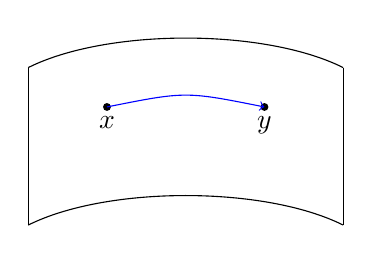
\begin{tikzpicture}
        \draw (-2,1) .. controls (-1,1.5) and (1,1.5) .. (2,1);
        \draw (-2,-1) .. controls (-1,-0.5) and (1,-0.5) .. (2,-1);
        \draw (-2,-1) -- (-2,1);
        \draw (2,-1) -- (2,1);
        \fill (-1,0.5)node[below]{$x$} circle (0.05);
        \fill (1,0.5)node[below]{$y$} circle (0.05);
        \draw[->,blue] (-1,0.5) .. controls (0,0.7) .. (1,0.5);
    \end{tikzpicture}    
\end{center}
所有把$x$移动到$y$的群元素构成群$G$关于子群$G_x$的陪集,流形上每一点$y$都对应一个陪集,所以$G/G_x\sim \mathcal{M}$
\subsection{Grassmannian流形}
在数学上,Grassmannian流形$Gr(k, V)$是一个参数化$n$维向量空间$V$的所有$k$维线性子空间的集合。例如,Grassmannian流形$Gr(1, V)$是通过$V$中原点直线构成的集合,因此它与比$V$低一维的射影空间相同。

当$V$是实向量空间或复向量空间时,Grassmannian流形是紧致光滑流形。一般来说,它们具有平滑代数簇的结构,维数为$k(n-k)$

给出Grassmannian一个几何结构的最快方法是把它表示为一个齐次流形。首先,回想一下一般线性群$GL(V)$作用于$V$的$r$维子空间。因此如果在这个作用下$H$是不动子空间,我们有
\begin{equation}
    Gr(r,V)=GL(V)/H
\end{equation}
如果数域$V$是$R$或$C$,并且$GL(V)$被认为是一个李群,那么这种构造使Grassmannian变成一个光滑流形。也可以使用其他群来构建这种结构。为了做到这一点,在$V$上固定一个内积。在$R$上,用正交群$O(V)$代替$GL(V)$,通过限制在正交坐标系中,就得到了恒等式
\begin{equation}
    \mathbf{G r}(r,\mathbb{R}^n)=\mathrm{O}(n) /(\mathrm{O}(r) \times \mathrm{O}(n-r))
\end{equation}
特别地,Grassmannian的维数是$r(n−r)$

在$C$上,用$U(V)$群代替$GL(V)$。这表明格拉斯曼是紧致的。这些结构也使格拉斯曼成为一个度量空间:对于$V$的子空间$W$,令$P_W$是$V$向$W$的投影算符,则有
\begin{equation}
    d(W,W')=\|P_W-P_{W'}\|
\end{equation}
其中$\|\cdot\|$表示算符的范数。时候$Gr(r,V)$上的度量。所用的内积并不重要,因为不同的内积会给出$V$上的一个等价范数,从而给出一个等价度规。

\begin{enumerate}
    \item $CP^n$:通过$\mathbb{C}^{n+1}$原点的复直线的集合。作用于$CP^n$上的传递群为$SU(n+1)$,它把复直线映射到复直线,迷向子群为$U(n)\times U(1)$,它不改变复直线
    \begin{equation}
        CP^n\simeq SU(n+1)/(U(n)\times U(1))\simeq S^{2n+1}/U(1)\simeq C^{n}\cup \{\infty\}
    \end{equation}
    当$n=1$时,$CP^1\simeq SU(2)/U(1)\simeq S^3/U(1)\simeq S^2$
    \item $RP^n$:通过$\mathbb{R}^{n+1}$原点实直线的集合。作用于$RP^n$上的传递群为$SO(n+1)$,迷向子群为$O(n)\times Z_2$.(这里注意$O(1)\simeq Z_2$) 即
    \begin{equation}
        RP^n\simeq SO(n+1)/(O(n)\times Z_2)\simeq S^n/Z_2
    \end{equation}
    \item 一般实Grassmannian流形:$R^n$中所有过原点的$k$维子空间的集合叫做Grassmannian流形$G(k,\mathbb{R}^n)$,它是正交群的陪集流形
    \begin{equation}
        G(k,\mathbb{R}^n) \simeq O(n) / (O(n-k) \times O(k))
    \end{equation}
    是$k(n-k)$维紧致连通流形
    \item 一般复Grassmannian流形:$C^n$中所有过原点的复$k$维子空间的集合叫做Grassmannian流形$G(k,\mathbb{C}^n)$,它是$U(n)$群的陪集流形
    \begin{equation}
        G(k,\mathbb{C}^n) \simeq U(n) / (U(n-k) \times U(k))
    \end{equation}
\end{enumerate}

\subsection{Stiefel流形}
在数学上Stiefel流形$V_k(\mathbb{R}^n)$是在$\mathbb{R}^n$上所有过原点$k$维正交标架的集合。也就是说,它是$\mathbb{R}^{n}$中向量的有序正交$k$元组的集合。类似的,可以在$\mathbb{C}^n$中的$k$维复正交标架定义复Stiefel流形$V_k(\mathbb{C}^n)$. 同样的在四元数空间$\mathbb{H}^n$上也可以定义$V_k(\mathbb{H}^n)$. 更一般地,这种构造适用于任何实、复或四元内积空间。

令$\mathbb{F}$表示$\mathbb{R},\mathbb{C},\mathbb{H}$. Stiefel流形$V_k(\mathbb{F}^n)$可以被看成一个$n\times k$的矩阵集合,其中把$k$标架写成$\mathbb{F}^n$中$k$列向量排成的矩阵。正交关系可以写成$A^{\dagger}A=I_k$,其中$A^\dagger$表示转置共轭,$I_k$表示$k\times k$的单位矩阵。所以有
\begin{equation}
    V_k(\mathbb{F}^n)=\{A\in\mathbb{F}^n|A^\dagger A=I_k\}
\end{equation}
\begin{equation}
    \begin{aligned}
    \operatorname{dim} V_{k}\left(\mathbb{R}^{n}\right) &=n k-\frac{1}{2} k(k+1) \\
    \operatorname{dim} V_{k}\left(\mathbb{C}^{n}\right) &=2 n k-k^{2} \\
    \operatorname{dim} V_{k}\left(\mathbb{H}^{n}\right) &=4 n k-k(2 k-1)
    \end{aligned}
\end{equation}
每个Stiefel流形$V_{k}(\mathbb{F}^{n})$都可以被视为经典群以自然方式作用的齐次空间。

在$\mathbb{R}^{n}$中,$k$标架的每一个正交变换都会得到另一个$k$标架,并且任意两个$k$标架通过某些正交变换相互关联。换句话说,正交群$O(n)$在$V_k(\mathbb{R}^n)$上作用传递。给定标架的迷向子群同构于$O(n-k)$,$O(n−k)$非平凡地作用于该坐标系所生成空间的正交补。

同样的$U(n)$对于$V_k(\mathbb{C}^n)$作用传递,迷向子群是$U(n-k)$. 辛群$Sp(n)$对于$V_k(\mathbb{H}^n)$作用传递,迷向子群是$Sp(n-k)$

所以$V_k(\mathbb{F}^n)$可以被看成一个齐性流形
\begin{equation}
    \begin{aligned}
    V_{k}\left(\mathbb{R}^{n}\right) & \cong \mathrm{O}(n) / \mathrm{O}(n-k) \\
    V_{k}\left(\mathbb{C}^{n}\right) & \cong \mathrm{U}(n) / \mathrm{U}(n-k) \\
    V_{k}\left(\mathbb{H}^{n}\right) & \cong \mathrm{Sp}(n) / \mathrm{Sp}(n-k)
    \end{aligned}
\end{equation}
当$k=n$时,对应于作用自由,Stiefel流形$V_k(\mathbb{F}^n)$是对应经典群的一个主齐次空间。

当$k$严格小于$n$时,$SO(n)$也对$V_k(\mathbb{R}^n)$作用传递,迷向子群是$SO(n-k)$
\begin{equation}
    V_{k}\left(\mathbb{R}^{n}\right) \cong \operatorname{SO}(n) / \mathrm{SO}(n-k) \quad \text { for } k<n
\end{equation}
对于$V_k(\mathbb{C}^n)$同样成立
\begin{equation}
    V_{k}\left(\mathbb{C}^{n}\right) \cong \mathrm{SU}(n) / \mathrm{SU}(n-k) \quad \text { for } k<n
\end{equation}
因此,对于$k = n−1$,Stiefel流形是相应的特殊经典群的主齐次空间。




\end{document}